%\documentclass[iop]{emulateapj}
\documentclass[aps, pre, onecolumn, nofootinbib, notitlepage, groupedaddress, amsfonts, amssymb, amsmath, longbibliography]{revtex4-1}
\usepackage{tabularx}
\usepackage{graphicx}
\usepackage{hyperref}
\usepackage{xcolor}
\hypersetup{
    colorlinks,
    linkcolor={red!50!black},
    citecolor={blue!50!black},
    urlcolor={blue!80!black}
}
\usepackage{bm}
\usepackage{natbib}
\usepackage{longtable}
\LTcapwidth=0.87\textwidth

\newcommand{\Div}[1]{\ensuremath{\nabla\cdot\left( #1\right)}}
\newcommand{\DivU}{\ensuremath{\nabla\cdot\bm{u}}}
\newcommand{\angles}[1]{\ensuremath{\left\langle #1 \right\rangle}}
\newcommand{\grad}{\ensuremath{\nabla}}
\newcommand{\RB}{Rayleigh-B\'{e}nard }
\newcommand{\stressT}{\ensuremath{\bm{\bar{\bar{\Pi}}}}}
\newcommand{\lilstressT}{\ensuremath{\bm{\bar{\bar{\sigma}}}}}
\newcommand{\nrho}{\ensuremath{n_{\rho}}}
\newcommand{\approptoinn}[2]{\mathrel{\vcenter{
	\offinterlineskip\halign{\hfil$##$\cr
	#1\propto\cr\noalign{\kern2pt}#1\sim\cr\noalign{\kern-2pt}}}}}

\newcommand{\appropto}{\mathpalette\approptoinn\relax}

\newcommand\mnras{{MNRAS}}%

\begin{document}
\author{Evan H. Anders}
\affiliation{Dept. Astrophysical \& Planetary Sciences, University of Colorado -- Boulder, Boulder, CO 80309, USA}
\affiliation{Laboratory for Atmospheric and Space Physics, Boulder, CO 80303, USA}
\author{Benjamin P. Brown}
\affiliation{Dept. Astrophysical \& Planetary Sciences, University of Colorado -- Boulder, Boulder, CO 80309, USA}
\affiliation{Laboratory for Atmospheric and Space Physics, Boulder, CO 80303, USA}
\author{Jeffrey S. Oishi}
\affiliation{Department of Physics and Astronomy, Bates College, Lewiston, ME 04240, USA}
\title{Accelerated evolution of convective simulations}

\begin{abstract}
We present a method for coupling boundary value problems with initial value problems 
in order to achieve Accelerated Evolution (AE) of convective solutions on
dynamical timescales, rather than the long thermal timescale. 
We study this method in the context of \RB convection. 
We demonstrate that the solution reached by AE and Standard Evolution (SE) are
similar, and that this method works at a
large range of supercriticalities.  The AE method is used to achieve converged 
solutions at high supercriticality ($10^7$), and its extensions to more complex 
systems are briefly discussed.
\end{abstract}
\maketitle

%%%%%%%%%%%%
%%%%%%%%%%%
% INTRO
%%%%%%%%%%%
%%%%%%%%%%%%

\section{Introduction}
\label{sec:intro}
Natural convection occurs in the presence of disparate timescales which
prohibit numericists from studying realistic models of natural systems.  For example,
flows in the convection zones of stars like the Sun are characteristically low Mach number
(Ma) in the deep interior.
Explicit timestepping methods which are bound by the Courant-Friedrich-Lewy
(CFL) timestep limit must resolve the fastest motions (sound
waves), resulting in timesteps which are prohibitively
small for studies of the deep, low-Ma motions. These systems are numerically
stiff, and the difference between
the sound crossing time and the convective overturn time have made studies of low-Ma stellar
convection difficult. Traditionally, approximations such as
the anelastic approximation, in which sound waves are explicitly filtered out,
have been used to study low-Ma flows \cite{brown&all2010, featherstone&hindman2016}.
More recently, advanced numerical techniques which use implicit or mixed
implicit-explicit timestepping mechanisms have made it feasible to study
convection at low Mach numbers \cite{viallet&all2011, viallet&all2013, viallet&all2016, lecoanet&all2014,
anders&brown2017, bordwell&all2018}, and careful studies of deep convection which
would have been impossible a decade ago are now widely accessible.

Convective systems with divergent dynamical timescales can now be studied; however,
thermal timescales, which characterize system relaxation, are often much larger than
dynamical timescales, and resolving dynamics in atmospheres which are sufficiently
thermally relaxed remains a challenging problem.
Solar convection is a prime example of this phenomenon.
Dynamical timescales in the solar convective zone are relatively short 
(10 min overturn at solar surface, one month solar
rotation rate) compared to the Sun's Kelvin-Helmholtz timescale of
$3 \cdot 10^7$ years \cite{stix2003}.  
In such a system, it is impossible to resolve the convective dynamics while also
evolving the thermal structure of the system in a meaningful fashion using
traditional timestepping techniques alone.
As modern simulations aim to model natural convection
by increasing into the high-Rayleigh-number (Ra) regime,
the thermal diffusion timescale becomes intractably large
compared to dynamical timescales \cite{anders&brown2017}.
Furthermore, as dynamical and thermal timescales separate, 
simulations become more turbulent. Increasingly turbulent motions 
require finer grid meshes and smaller timesteps
to capture advective dynamics. Thus, the progression of simulations into the high-Ra
regime of natural convection is slowed by two simultaneous effects: timestepping
through a single convective overturn time becomes more computationally expensive
and the number of overturn times required for systems to reach thermal equilibration
grows.

The vast difference between convective and thermal timescales has long plagued
numericists studying convection, and an abundance of approaches has been employed to
study thermally converged solutions. One popular method for accelerating the convergence
of high-Ra solutions is by ``bootstrapping'' -- the process of using the flow
fields in a converged solution at low Ra as initial conditions for a simulation at high
Ra.  This method has been used with great success \cite{johnston&doering2009, verzicco&camussi1997},
but it is not without its faults.  Bootstrapped solutions are succeptible to hysteresis
effects, in which large-scale convective structures present in the
low Ra solution imprint onto the dynamics of the new, high Ra solution. 
Another commonly-used tactic in
moderate-Ra simulations is to use 
a simple model of the full convective state as initial conditions.  
For example, past studies have used a linear eigenvalue solve to set the initial
convective state \cite{hurlburt&all1984} or used an axisymmetric solution 
as initial conditions for convection in a 3D cylinder \cite{verzicco&camussi1997}. 
In other systems, 
the approximate state of the evolved solution can be estimated. There, a
set of initial conditions which is close to the evolved state be 
derived analytically \cite{couston&all2017, brandenburg&all2005}.

Despite the numerous methods that have been used,
the most straightforward way to achieve a thermally converged solution
is to evolve a convective simulation through a thermal timescale. Some modern
studies do just that \cite{featherstone&hindman2016}.
However, such evolution is
\emph{expensive}, and state-of-the-art simulations at the highest values of Ra
can only reasonably be run
for tens to hundreds of buoyancy times \cite{stevens&all2011}, much less the
thousands of buoyancy timescales required for thermal convergence.

In this work, we study a method of achieving accelerated evolution of
convective simulations. We couple measurements of the dynamics of non-converged
convective simulations with knowledge about energy balances in the desired solution
to self-consistently adjust the mean thermodynamic profile towards its evolved state. 
While such a method has been used previously \cite{hurlburt&all1986}, 
we find no explanation in the current literature of the steps involved in employing
this method, nor any study into the accuracy of such a method.
In section \ref{sec:experiment}, we describe our convective simulations, our
numerical methods, and our method for achieving accelerated evolution. In
section \ref{sec:results}, we compare solutions reached through the accelerated evolution
method to those that have been evolved through a full diffusive timescale, and we
examine select simulations at high Ra which have achieved accelerated evolution. Finally,
in section \ref{sec:extensions}, we discuss extensions of the methods presented here,
and we offer concluding remarks.


%%%%%%%%%%%%
%%%%%%%%%%%
% EXPERIMENT
%%%%%%%%%%%
%%%%%%%%%%%%

\section{Experiment}
\label{sec:experiment}
We study incompressible \RB convection under the Oberbeck-Boussinesq approximation,
such that our fluid
has a constant kinematic viscosity ($\nu$), thermal diffusivity ($\kappa$), and coefficient
of thermal expansion ($\alpha$). The density of the fluid is a constant, $\rho_0$,
except where it is $\rho = \rho_0(1  - \alpha T_1)$ on the term where
the constant gravitational acceleration, $\bm{g} = - g\hat{z}$, 
acts in the vertical momentum equation.
The equations of motion are \cite{spiegel&veronis1960}
\begin{gather}
\DivU = 0, 
	\label{eqn:incompressible}
\\
\frac{\partial \bm{u}}{\partial t} + \bm{u}\cdot\grad\bm{u} =
-\frac{1}{\rho_0}\grad P - g( 1 - \alpha T_1)\hat{z} + \nu\grad^2\bm{u}, 
	\label{eqn:dim_bouss_momentum}
\\
\frac{\partial T_1}{\partial t} + \bm{u}\cdot\grad(T_0 + T_1) = \kappa\grad^2 T_1,
	\label{eqn:dim_bouss_energy}
\end{gather}
where $\bm{u} = u\hat{x} + v\hat{y} + w\hat{z}$ is the velocity, 
$T = T_0 + T_1$ are the initial and fluctuating components of temperature, 
and $P$ is the pressure.
We non-dimensionalize these equations such that the
length is in units of the layer height ($L_z$),
temperature is in units of the initial temperature jump across the layer ($\Delta T_0 = L_z \grad T_0$), 
and velocity is in units of the freefall velocity ($v_{\text{ff}} = \sqrt{\alpha g L_z^2 \grad T_0}$).
by these choices, one time unit is a freefall time ($L_z/v_{\text{ff}}$).
We introduce a reduced kinematic pressure,
$\varpi \equiv (P / \rho_0 + \phi + |\bm{u}|^2 / 2) / v_{\text{ff}}^2$, where the gravitational
potential, $\phi$, is defined such that $\bm{g} = -\grad \phi$. As $P$ is a
Langrange multiplier under the Oberbeck-Boussinesq approximation, $\varpi$
can be treated straightforwardly as a linear variable. 
In non-dimensional form, Eqns. \ref{eqn:dim_bouss_momentum} \& \ref{eqn:dim_bouss_energy}
become
\begin{gather}
\frac{\partial \bm{u}}{\partial t} + \grad \varpi - T_1\hat{z} + \mathcal{R}\grad\times\bm{\omega} = \bm{u}\times\bm{\omega},
	\label{eqn:bouss_momentum}
\\
\frac{\partial T_1}{\partial t} - \mathcal{P}\grad^2 T_1 + w \frac{\partial T_0}{\partial z} = - \bm{u}\cdot\grad T_1,
	\label{eqn:bouss_energy}
\end{gather}
where $\bm{\omega} = \grad \times \bm{u}$ is the vorticity.
The dimensionless control parameters $\mathcal{P}$ and $\mathcal{R}$ 
are set by the Rayleigh and Prandtl numbers,
\begin{equation}
\mathcal{R} \equiv \sqrt{\frac{\text{Pr}}{\text{Ra}}}, \qquad \mathcal{P} \equiv \frac{1}{\sqrt{\text{Pr}\,\text{Ra}}}, \qquad
\text{Ra} = \frac{g \alpha L_z^4 \grad T_0}{\nu\kappa} = \frac{(L_z\,v_{\text{ff}})^2}{\nu\kappa}, \qquad \text{Pr} = \frac{\nu}{\kappa}.
\end{equation}
We hold Pr$ = 1$ constant throughout this work, such that $\mathcal{P} = \mathcal{R}$.

We study 2D and 3D convection in which the domain is a cartesian box, 
whose dimensionless vertical extent is $z \in [-1/2, 1/2]$, 
and which is horizontally periodic with an extent of $x, y \in [0, \Gamma]$,
where $\Gamma = 2$ is the aspect ratio. 
In 2D simulations, we set $v = \partial_y = 0$.
We specify no-slip, impenetrable boundary conditions at both the top and
bottom boundary and we use mixed thermal boundary conditions, such that
\begin{equation}
u = v = w = 0 \, \, \text{at}\,\,z = \pm 1/2, \qquad T_1 = 0 \,\,\text{at}\,\, z=+1/2, \qquad
\frac{\partial T_1}{\partial z} = 0\,\,\text{at}\,\,z=-1/2.
\label{eqn:bcs}
\end{equation}
For this choice of boundary conditions, the critical value of Ra at which
the onset of convection occurs is Ra$_{\text{crit}} = 1295.78$, and the
supercriticality of a run is defined as $S \equiv \text{Ra}/\text{Ra}_{\text{crit}}$.
Studies of convection which aim to model
astrophysical systems such as stars often employ mixed thermal
boundary conditions \cite{hurlburt&all1984, cattaneo&all1991, korre&all2017},
as we do here; however, our choice of thermal boundary conditions here
reflects the fact that the conditions in Eqn. (\ref{eqn:bcs}) are the simplest
to implement in the process of accelerated evolution (see section \ref{subsection:ae})
we study here.

We utilize the 
Dedalus\footnote{\url{http://dedalus-project.org/}} 
pseudospectral framework \cite{burns&all2016} to evolve  
Eqns. (\ref{eqn:incompressible}), (\ref{eqn:bouss_momentum}), \& (\ref{eqn:bouss_energy}) 
forward in time
using an implicit-explicit (IMEX), third-order, four-step 
Runge-Kutta timestepping scheme RK443 \cite{ascher&all1997}.  
The linear terms (on the LHS of the equations) are solved implicitly,
while the nonlinear terms (RHS) are explicitly solved.
Variables are time-evolved on a dealiased Chebyshev (vertical)
and Fourier (horizontal, periodic) domain in which the
physical grid dimensions are 3/2 the size of the coefficient grid.  

As initial conditions, we fill $T_1$ with
random white noise whose magnitude is $10^{-6}\mathcal{P}$.
This ensures that the initial perturbations are much smaller than the
evolved convective temperature perturbations, even at large Ra.
We filter this noise spectrum in coefficient space, 
such that only the lower 25\% of the coefficients
have power.


%%%%%%%%%%%%
%%%%%%%%%%%
% AE METHOD
%%%%%%%%%%%
%%%%%%%%%%%%

\subsection{The method of Accelerated Evolution}
\label{subsection:ae}
Here we describe a method of Accelerated Evolution (AE), which we use 
to rapidly evolve the thermodynamic state of convective simulations.  
We compare this AE method to Standard Evolution
(SE), in which we naively evolve the atmosphere for one thermal diffusion time,
$t_\kappa = \mathcal{P}^{-1}$. As Ra increases, SE solutions become intractable, 
while the timeframe of convergence for an AE solution remains nearly constant
in freefall time units.
For an example of time saving achieved by using AE, we compare
energy traces at $S = 10^5$ from a SE run in Fig. \ref{fig:time_trace}a to an AE run
in Fig. \ref{fig:time_trace}c.

The horizontally averaged profiles of the vertical conductive flux, 
F$_{\text{cond}} = \angles{-\kappa\grad(T_0 + T_1)}_{x,y}$, and the vertical convective flux,
F$_{\text{conv}} = \angles{w(T_0 + T_1)}_{x,y}$, where $\angles{}_{x,y}$ represent
a horizontal average, are the basis of the AE method. We measure
both of these quantities early in a simulation, retrieving profiles similar to
those shown in Fig. \ref{fig:time_trace}b.
At early stages in the simulation, these flux profiles are highly asymmetric,
with more flux exiting the atmosphere at the upper boundary than 
the fixed-flux lower boundary is providing.
By calculating the total flux,
F$_{\text{tot}} =$ F$_{\text{conv}} +$ F$_{\text{cond}}$, we derive the profiles
\begin{equation}
f_{\text{conv}}(z) = \frac{F_{\text{conv}}}{F_{\text{tot}}},\qquad
f_{\text{cond}}(z) = \frac{F_{\text{cond}}}{F_{\text{tot}}},
\label{eqn:bvp_ratios}
\end{equation}
which have the systematic asymmetries removed. These profiles describe which
parts of the atmosphere depend on convection to carry flux (where $f_{\text{conv}}(z) = 1$
and $f_{\text{cond}}(z) = 0$).
We presume that the early convection occupies roughly the same volume as the evolved
convection, and thus that the extent of the early thermal boundary layers 
(where $f_{\text{cond}}(z) = 1$ and $f_{\text{conv}}(z) = 0$) 
will not change significantly over the course of the atmosphere's evolution.
Under this assumption, the proper evolved atmospheric flux profiles
are F$_{\text{conv, ev}} = \text{F}_{\text{bot}}\cdot f_{\text{conv}}$
and F$_{\text{cond, ev}} = \text{F}_{\text{bot}}\cdot f_{\text{cond}}$,
where F$_{\text{bot}} = \mathcal{P}$ is the amount of flux entering the
bottom of the atmosphere.

\begin{figure*}[t!]
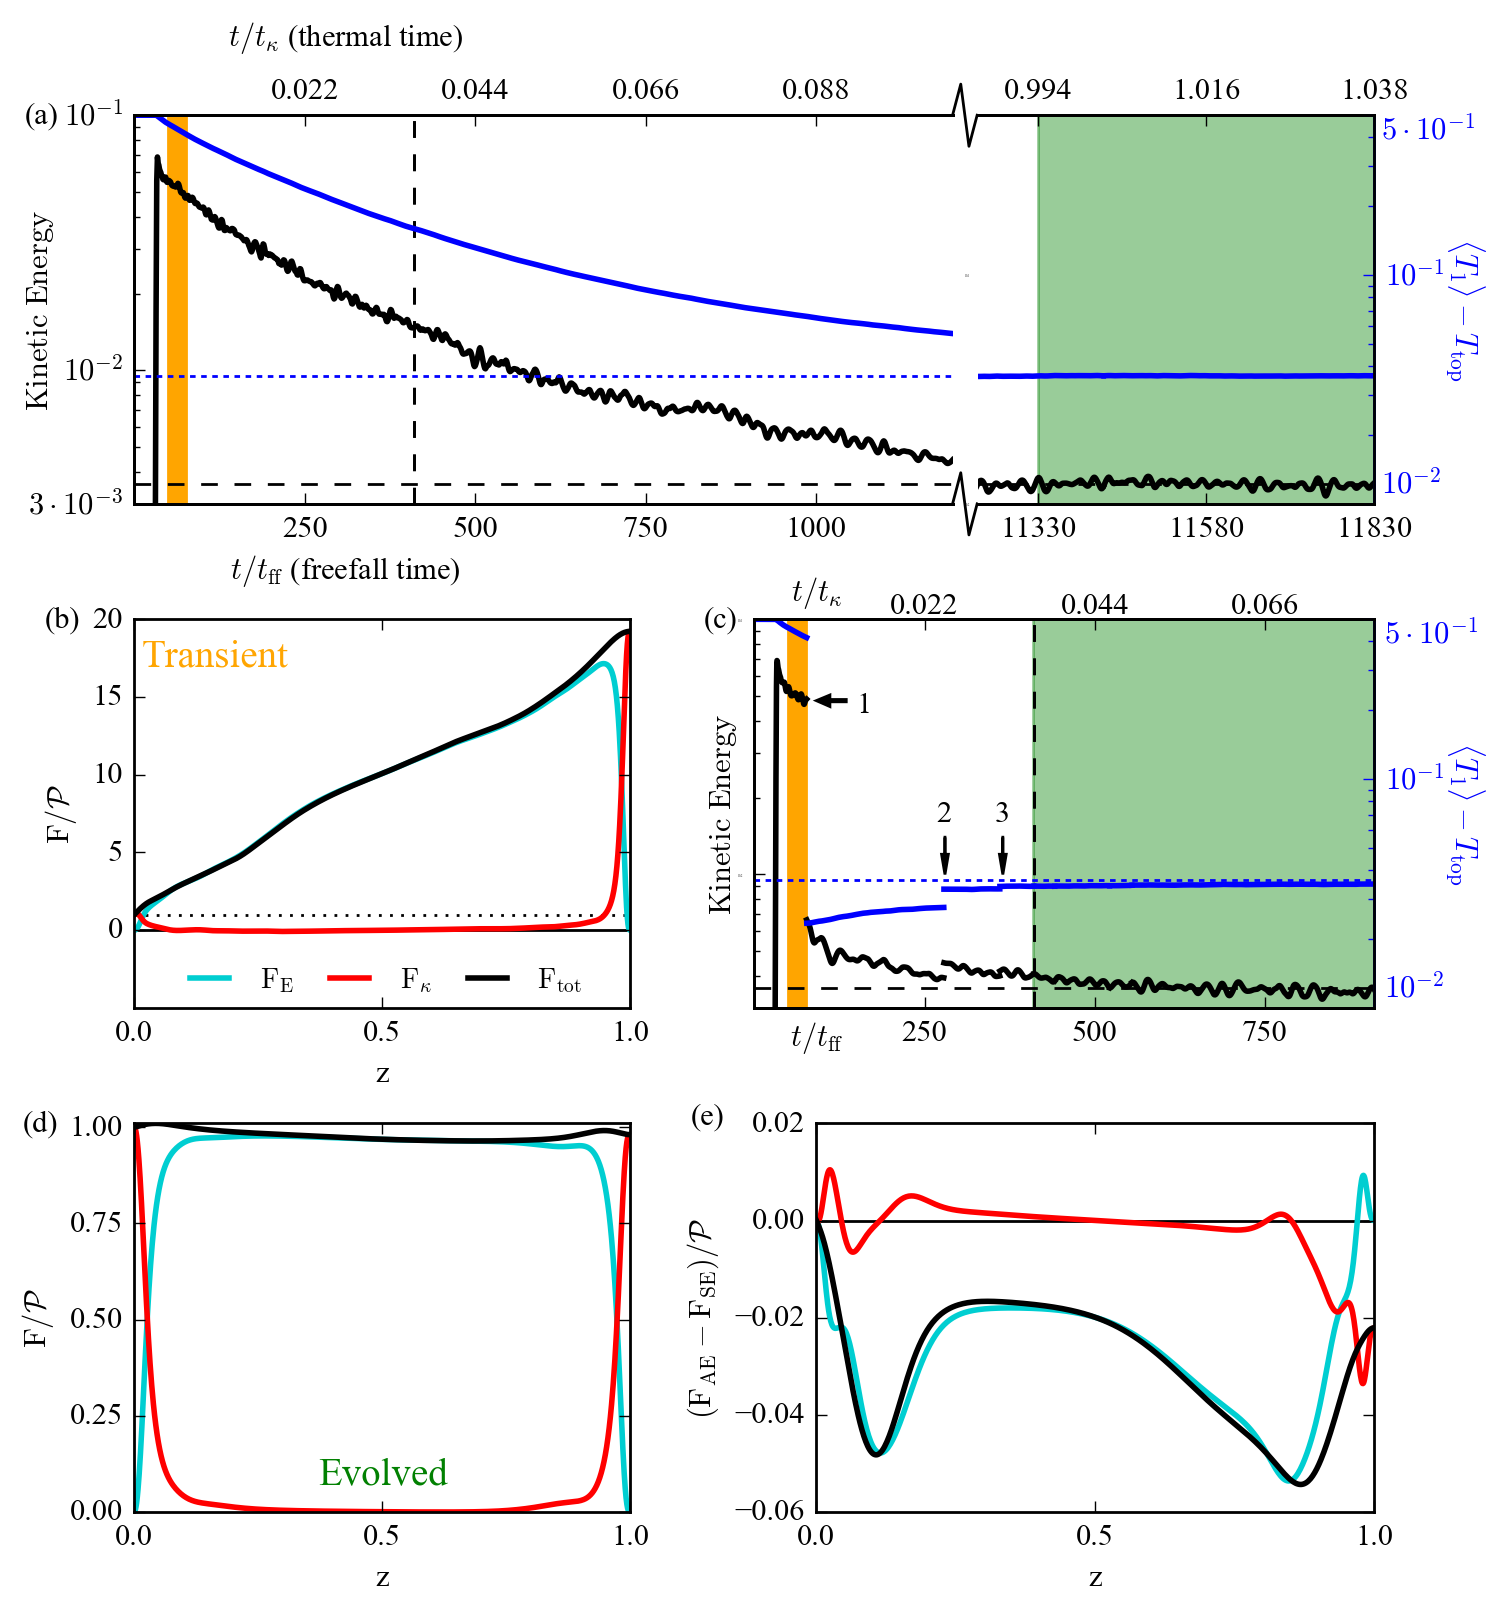
\includegraphics[width=\textwidth]{./figs/time_trace.png}
\caption{(a) Kinetic energy (black) and mean temperature (blue)  vs. time are shown
for a SE run at $S = 10^5$. The mean evolved values of kinetic energy and mean temperature,
averaged over the time shaded in green,
are denoted by the horizontal dashed lines. (b) The time- and horizontally-averaged
flux profiles are shown for the times highlighted in orange in (a).
(c) The same quantities as in (a) are shown, but for AE at the same parameters.
The axes are scaled identically in (a) and (c), and the AE method is used three times, marked by
the numbered arrows in (c). The fluxes averaged over the green shaded region of (c)
are shown in (d). The difference between
the fluxes in the AE and SE solutions is shown in (e). The dashed
vertical line in (a) and (c) denotes the simulation time at which evolved measurements
are started for the AE case.
\label{fig:time_trace} }
\end{figure*}

In a time-stationary state, the horizontal- and time-average of
Eqns. (\ref{eqn:bouss_momentum}) and (\ref{eqn:bouss_energy}), neglecting terms which
vanish due to symmetry, are
\begin{gather}
\frac{\partial}{\partial z}\angles{\varpi}_{x,y} - \angles{T_1}_{x,y}\hat{z} = \angles{\bm{u}\times\bm{\omega}}_{x,y},
	\label{eqn:bouss_BVP_momentum}
\\
\frac{\partial}{\partial z}\text{F}_{\text{conv, ev}} - \mathcal{P}\frac{\partial^2}{\partial z^2} \angles{T_1}_{x,y} = 0.
	\label{eqn:bouss_BVP_energy}
\end{gather}
Convective flows
are perturbations around a thermal profile defined by these equations in the proper evolved, 
statistically stationary state. Furthermore, under the specification of
F$_{\text{conv, ev}}$ and $\angles{\bm{u}\times\bm{\omega}}_{x,y}$,
\emph{the mean thermodynamic structure of the system is fully specified}.

Thus, the AE method is simple: we construct F$_{\text{conv, ev}}$ as described above.
Then we calculate a profile, 
$\xi(z) = \text{F}_{\text{conv, ev}}/\text{F}_{\text{conv}}$, which is the fraction,
as a function of height, by which the flux in the system must be reduced to go from
an initial state (Fig. \ref{fig:time_trace}b) to an evolved state (Fig. \ref{fig:time_trace}d).
We multiply the velocities
and the thermal fluctuations, $T - \angles{T}_{x,y}$, by $\sqrt{\xi}$, such 
that the advected, flux-carrying perturbations in the temperature are appropriately
diminished.  We then solve a boundary value problem including
Eqns. (\ref{eqn:bouss_BVP_momentum}) \& (\ref{eqn:bouss_BVP_energy}) using F$_{\text{conv, ev}}$
and $\cdot\angles{\bm{u}\times\bm{\omega}}_{x,y}$, after diminishing it by a factor
of $\xi$. We use mixed thermal boundary conditions, as in Eqn. (\ref{eqn:bcs}),
because $F_{\text{bot}}$ is exactly specified, and the temperature profile is pegged
at a reference value for the AE solve.
For specifics on the precise implementation of the AE method, we refer
the reader to appendix \ref{appendix:recipe}.

The AE method converges atmospheres from extreme flux disequilibrium states 
(Fig. \ref{fig:time_trace}b) on short dynamical timescales (Fig. \ref{fig:time_trace}c)
to a converged state (Fig. \ref{fig:time_trace}d) whose flux balance is very
close to the balance present in the corresponding SE solution (Fig. \ref{fig:time_trace}e).
While the application of the AE method advances solutions toward the proper solution,
we find that multiple applications of the method is the best means of achieving converged
solutions quickly.


%%%%%%%%%%%%
%%%%%%%%%%%
% RESULTS
%%%%%%%%%%%
%%%%%%%%%%%%

\section{Results}
\label{sec:results}
We study evolved solutions achieved through the standard evolution (SE) method 
from convective onset
up to $S = 10^5$ in 2D and $S = 10^4$ in 3D.  These SE runs are compared to
accelerated evolution (AE) runs spanning from onset up to $S = 10^7$ in 2D and $S = 10^4$ in 3D.
For a full list of simulations, we refer the reader to appendix \ref{appendix:run_table}.

We report the time- and volume-averaged values of select measurements of the
evolved solutions in Fig. \ref{fig:parameter_space_comparison}.
The scaling of heat transport in the evolved solution, as quantified by the
Nusselt number, is shown in Fig. \ref{fig:parameter_space_comparison}a.
The volume averaged Nusselt number is defined as
\begin{equation}
\text{Nu} = \frac{\angles{F_{\text{conv}} + F_{\text{cond}}}}{\angles{F_{\text{cond, ref}}}}
 = \frac{\angles{wT - \mathcal{P}\partial_z T}}{\angles{- \mathcal{P} \partial_z T}},
\end{equation}
where $\angles{}$ represent a volume average.
In 2D when $S < 10^{3+2/3}$ and in 3D, the evolved system is defined by a clear
value of Nu and the convective heat transport reaches a temporally stationary state.
In 2D and at larger values of $S$, the value of Nu oscillates as a function of time
due to large horizontal oscillations in the convective plume structures.
Our choice of no-slip
boundary conditions prevent the fluid from entering a shearing state
\cite{goluskin&all2014}, but the oscillatory motions which do arise cause the
system to vary between periods of low heat transport and high heat transport.
The SE simulations which span up to $S = 10^5$ exhibit the same horizontally
oscillatory motion as the AE solutions for the same initial conditions. The
scaling of the mean value of Nu is roughly $\text{Nu} \propto \text{Ra}^{1/5}$,
weaker than that reported in similar systems with fixed-T and fixed-flux boundary
conditions \cite{johnston&doering2009}.  We attribute this weaker Nu scaling to
the oscillatory nature of the plumes, which may have been avoided by previous studies
using bootstrapping techniques as initial conditions.

\begin{figure}[b]
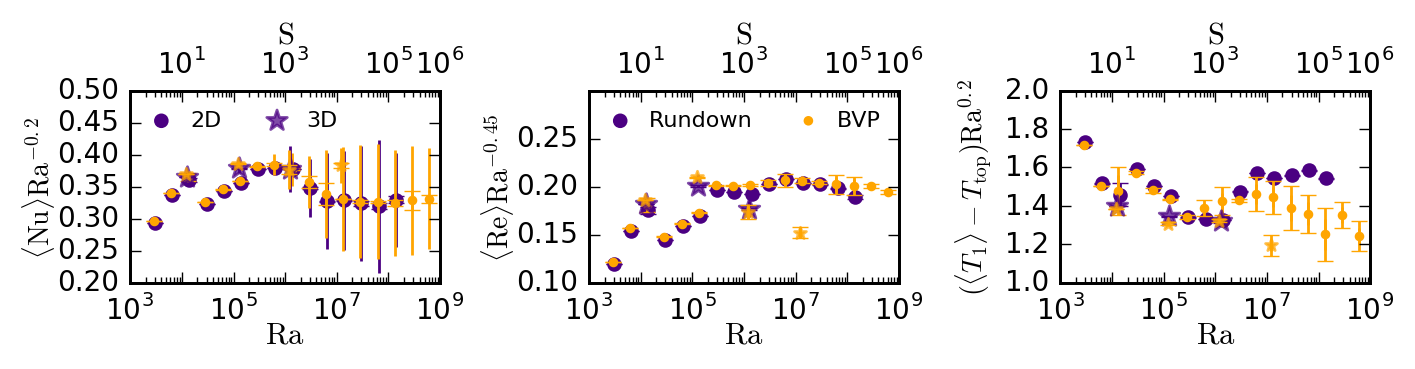
\includegraphics[width=\textwidth]{./figs/parameter_space_comparison.png}
\caption{Volume- and time-averaged measurements of the Nusselt number (Nu), the
RMS Reynolds number (Re), and the mean temperature ($\angles{T}$) for AE runs are shown in (a)-(c).
Symbols are located at the mean value of
each measurement.  Vertical lines represent the standard deviation of the measurement,
and quantify natural variation over the
averaging window. Error bars represent the change in the mean value over the averaging window,
such that very large error bars represent solutions which are not fully converged when averaging
begins.
(a) Nu scales as Ra$^{1/5}$; above S$\geq 10^{3+2/3}$,
simulations exhibit oscillating plume structures whose heat transport fluctuates over time.  
(b) Re, which measures the level of turbulence in the evolved solution, scales as
Ra$^{0.45}$. (c) The difference between $\angles{T}$ and the value of $T$ at $z = +1/2$
is shown, and this quantity scales as Ra$^{-1/5}$, the inverse of Nu.
Relative error for measurements of (d) Nu, (e) Re, and (f) $T$ between 
AE solutions and SE solutions are shown.
The greyed area of the plots indicates the region in which only AE runs were
carried out due to computational expense. The run at $S = 10^5$ marked as a
black square is examined in more details in Figs. \ref{fig:time_trace},
\ref{fig:temp_comparison}, \& \ref{fig:pdf_comparison}.
\label{fig:parameter_space_comparison} }
\end{figure}



In Fig. \ref{fig:parameter_space_comparison}b, we report the volume-averaged
RMS Reynolds number in the AE solutions, where
$\text{Re} = \angles{|\bm{u}|} / \mathcal{R}$.  This measure scales roughly as
$\text{Re} \propto \text{Ra}^{0.45}$, and shows little variance with time.

In Fig. \ref{fig:parameter_space_comparison}c, we report the volume averaged 
temperature of the AE solutions, with the value at the upper (fixed $T$) boundary removed.
This measurement probes the thickness of the boundary layers of the solutions, and
should show scaling which is inversely proportional to Nu in converged solutions
where fixed-flux boundary conditions are used \cite{otero&all2002}.  We find here
that $(\angles{T} - T_{\text{top}}) \propto \text{Ra}^{-1/5}$, precisely the inverse
scaling of Nu, giving confidence that these solutions are in a converged state.

In Fig. \ref{fig:parameter_space_comparison}d-f, we report the fractional difference
between measurements from the AE solutions and measurements from the SE solutions.
We find that the mean value of Nu from AE solutions is accurate to the values
from SE solutions to within $\sim 1$\%, and the same is true for $\angles{T}$ measurements.
Re measurements show slightly greater error, with AE measurements being on average
$\leq 2$\% away from the SE measurements. 

The measurements presented in Fig. \ref{fig:parameter_space_comparison} demonstrate
that the AE method can be powerfully employed in parameter space studies in which
large numbers of simulations are compared in a volume-averaged sense.  We now turn
our examination to a more direct comparison of AE and SE for convection at
$S = 10^5$, as has been introduced in Fig. \ref{fig:time_trace}.

As the AE method primarily serves to adjust the thermodynamic structure of the
solution, we compare the temperature profile attained by AE and SE in 
Fig. \ref{fig:temp_comparison}.  We see that the boundary layer length scale is 
nearly identical between the two solutions (Fig. \ref{fig:temp_comparison}a), but that
the mean temperature in the interior differs by about 0.5\% on average
(Fig. \ref{fig:temp_comparison}c). 

\begin{figure}[t]
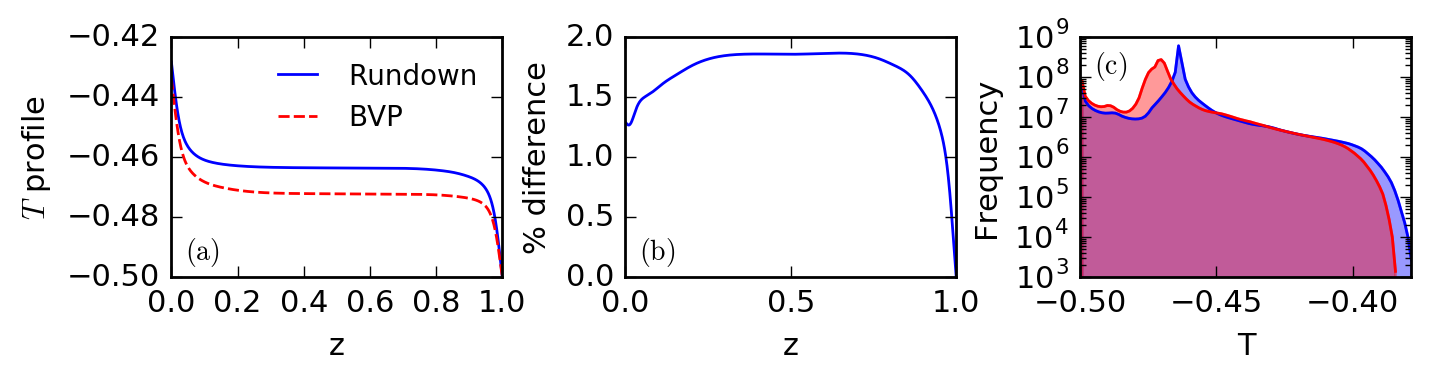
\includegraphics[width=\textwidth]{./figs/temp_comparison.png}
\caption{Comparisons of the evolved thermodynamic states of an AE and SE run
at $S = 10^{5}$ are shown.  (a) Evolved horizontally- and time-averaged 
temperature profiles, as a function of height.
(b) Probability Distribution Functions (PDFs) and their integrated
Cumulative Distribution Functions (CDFs)
of point-by-point measurements of the temperature field.
$T$ is sampled every 0.1 time units for 500 total time units,
and was interpolated onto an evenly spaced grid before sampling.
(c) The percentage difference between the mean temperature profiles as a function of height.
The difference between the mean profiles is very small, O(0.5\%).
(d) The value of the Kolmogorov-Smirnov (KS) statistic, or the difference between
the AE and SE CDFs, as a function of temperature.
The small
difference in the interior temperature 
results in a large difference between the two temperature CDFs near the values
of the temperature modes.  The spread of temperature around the modes, which includes the 
fluctuations that drive convection, are nearly identical between the two runs.
\label{fig:temp_comparison} }
\end{figure}



The probability distribution functions 
of point-by-point temperature measurements are compared for the two runs
in Fig. \ref{fig:temp_comparison}b.  We construct
this PDF from snapshots of the temperature profile every 0.1 freefall time
units over a duration of 500 total freefall time units, as shown by the green
areas if Fig. \ref{fig:time_trace}a\&c.  We interpolate the temperature field
of each of these snapshots onto an evenly spaced grid, determine the
frequency distribution of all measured $T$ values, and then normalize the
distribution such that its integral is unity.  The primary difference between
the two PDFs is their modes, which is expected from Fig. \ref{fig:temp_comparison}a. 
The fact that the the AE temperature
profile is roughly 0.5\% off of the SE temperature profile (\ref{fig:temp_comparison}c), 
the AE temperature
field is still marginally evolving towards the SE temperature field, and this
evolution appears as asymmetry of the AE PDF's peak.

One means of comparing two
probability distributions to determine if they are drawn from the same underlying
sample is through the use of a Kolmogorov-Smirnov (KS) \cite{wall&jenkins2012}.
In general, a KS test must be conducted on independent, uncorrelated data, which
poorly describes the point-by-point values of flow in a fluid simulation. Thus,
we will merely use the KS statistic, the maximum difference
between the cumulative distribution functions (CDFs) of the two sample distributions,
as a numerical method of directly comparing the two PDFs.  For the distributions
shown in Fig. \ref{fig:temp_comparison}b, the difference between the CDFs is shown
in Fig. \ref{fig:temp_comparison}d.  The maximum difiference, or the KS statistic,
is 0.495 near the modes.  This difference is very large, but is not unexpected.
While the temperature distributions near the modes are very different, their spread
of perturbations is nearly identical.


In addition to comparing the thermodynamic state achieved by the SE and AE methods,
we examine the velocities found in the evolved states.
We compute PDFs in the same manner as in Fig. \ref{fig:temp_comparison}b for the
vertical velocity (Fig. \ref{fig:pdf_comparison}a), horizontal velocity (Fig. \ref{fig:pdf_comparison}b),
and the nonlinear convective flux (Fig. \ref{fig:pdf_comparison}c). We report KS statistics
of 0.00615, 0.0349, and 0.0263, respectively.  Perhaps unsurpisingly, the nonlinear
convective transport between the SE and AE methods are very similar, as is captured
in a volume-averaged sense in the Nu measurements of Fig. \ref{fig:parameter_space_comparison}a\&d.
Each distribution shows a strong peak near zero due to the velocity boundary conditions
(Eqn. (\ref{eqn:bcs})), but the distribution of flux transport elements and velocities
is nearly identical in the AE and SE solutions.

\begin{figure}[t]
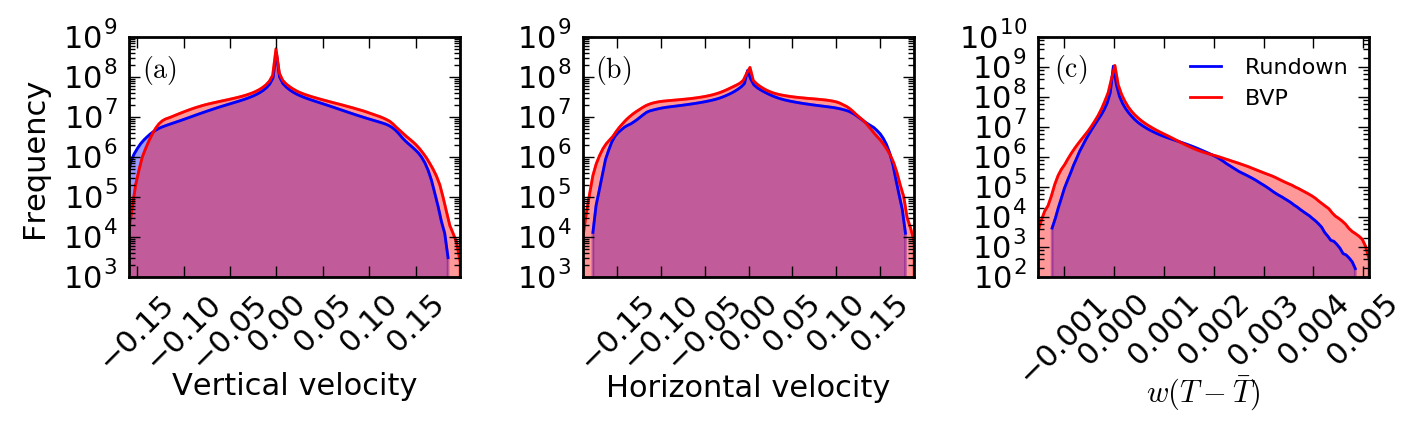
\includegraphics[width=\textwidth]{./figs/pdf_comparison.png}
\caption{Probability distribution functions (PDFs) of (a) the vertical velocity, (b) the horizontal velocity, and (c) nonlinear
convective transport are shown for 2D runs achieved through SE (blue) and AE (red)
at $S = 10^{5}$.  Flows are sampled every 0.1 time units for 500 total time units,
and are first interpolated onto an evenly spaced grid.
The cumulative distribution function (CDF) is overplotted for each PDF. 
(d-f) The KS statistics, or the values of CDF$_{\text{AE}}$ - CDF$_{\text{SE}}$,
are shown for the related distributions, and solid lines indicated positive values
while dashed lines are negative values. Unlike the temperature distributions in
Fig. \ref{fig:temp_comparison}, these distributions, particularly the vertical
velocity and transport, show very good agreement and small values of the KS statistic.
\label{fig:pdf_comparison} }
\end{figure}


The small differences between the SE and AE solutions for the case studied in 
Figs. \ref{fig:time_trace}, \ref{fig:temp_comparison}, \& \ref{fig:pdf_comparison},
show that the AE method is extremely powerful.  The first application of the AE method
($t \approx 70$ in Fig. \ref{fig:time_trace}b) immediately increases the 
average time step of our solver by a factor of 2-3. At higher supercriticality
($S = 10^7$), the AE solve immediately boosts the timestep by nearly a factor of 4.
Thus, not only does this method evolve the solution into nearly the correct state, 
but further time evolution (either to achieve precisely the correct thermodynamic
state or to take measurements of fluid quantities) happens more efficiently.


%%%%%%%%%%%%
%%%%%%%%%%%
% CONCLUSION
%%%%%%%%%%%
%%%%%%%%%%%%


\section{Extensions \& Conclusion}
\label{sec:extensions}
In this work, we have studied a method of Accelerated Evolution (AE) which can
be employed to achieve rapid thermal convergence of convective simulations.  We compared
this technique to the Standard Evolution (SE) of convection through a thermal diffusion timescale and
showed that AE rapidly obtains solutions whose dynamics are similar to SE solutions.
The AE method is not only valid at low values of $S$, where SE solutions
converge quickly due to the short thermal timescale, but AE is also applicable
at high values of $S$, where SE solutions are intractable.
We have studied
the AE method in both 2D and 3D, but restricted most of our study to 2D flows;
AE depends only on the 1D horizontal average of quantities, and our inclusion of 3D
simulations was merely to demonstrate the broadly useful nature of AE.

Here we studied \RB convection as a test case for the AE method, but we argue that
the true power of this technique is in its extensions to more complicated studies.
To achieve AE in more complicated systems, one need only derive 
the steady-state, horizontally-averaged equations governing
the convective dynamics
(e.g., Eqns. (\ref{eqn:bouss_BVP_momentum}) \& (\ref{eqn:bouss_BVP_energy}))
and couple those equations with knowledge of the boundary conditions
and current dynamics as described in
section \ref{subsection:ae} and appendix \ref{appendix:recipe}.
While in-depth studies of AE extensions are beyond the 
scope of this paper, we will briefly discuss
avenues in which the AE method should be explored and tested.

Convection in natural systems is often driven by internal heating processes
rather than imposed, fixed boundary condditions. The AE procedure can be straightforwardly
applied to Boussinesq studies of internally heated convection \cite{goluskin2016},
where a constant source term in the energy equation causes 
the vertical flux through the system to increase with height.
These systems can be straightforwardly
studied using exactly the methods that we examined here, but 
scaling the flux profiles derived
in Eqn. (\ref{eqn:bvp_ratios}) by the proper, height-dependent flux. Studies of
convection in natural system often employ height-dependent conductivities
\cite{brandenburg2016}, leading
to natural flux divergences that act as internal heating terms, and the study
of this method in the simple internal heating context will be an important step
towards achieving AE in simulations with astrophysically realistic conductivities.

In order to understand the influences of overshooting convection, some
studies examine adjacent stable and convecting regions
\cite{hurlburt&all1986, brandenburg&all2005, couston&all2017}.
When the interface between the stable region
and the convecting region is stiff and motions do not cross that interface,
convective motions cannot accelerate the restratification of the stable region.
In fully-convective domains, such as those studied in this work, the thermodynamics evolve
at a more rapid rate than the thermal diffusion time across the domain due to
the help of convective motions.  For example, in Fig. \ref{fig:time_trace}a,
the SE solution is fully converged after $4\cdot 10^3$ frefall time units,
despite the thermal timescale being roughly $10^4$ freefall units. However, in 
studies where there is a stable region which is not mixed by convection, the experimentalist
must either wait through a thermal diffusion time for the region to restratify
or employ methods such as the AE method to study evolved atmospheres.

Studies of stratified, compressible convection have much to gain through
developing and employing AE.
In many studies of stratified convection, the thermal diffusivity
is inversely proportional to the density \cite{anders&brown2017}. Thus, the
thermal timescale grows with depth in the atmosphere, and
the difficulty of achieving thermal convergence grows as simulators study more highly
stratified domains.
In order to extend AE into this regime, two additional pieces of information must be considered.
First, rather than constructing the profiles in Eqn. (\ref{eqn:bvp_ratios})
with the total flux through the domain, only the superadiabatic portion of
the flux should be considered.
Second, in addition to solving for
hydrostatic balance and thermal equilibrium, as in Eqns. (\ref{eqn:bouss_BVP_momentum})
\& (\ref{eqn:bouss_BVP_energy}), it is essential to simultaneously evolve the density
profile in a manner which conserves mass.  In a 1D boundary value problem, such as
is solved to achieve AE here, this implies the inclusion of an equation which tracks
the vertically integrated mass, and sets boundary conditions on that mass to ensure
that no mass enters or leaves the domain.  

An eventual use case of AE is in robustly replacing Mixing Length Theory (MLT)
in stellar evolution codes. Current state of the art stellar structure
models are the solutions of 1D simulations which parameterize convection 
using MLT \cite{paxton&all2011}. Recent work has taken the first steps towards
understanding how to simultaneously resolve convective motions while evolving
systems through many thermal timescales, as is required in the evolution of stars.
We now know that implicit timestepping methods, while not technically bound by
CFL constraints, must resolve the convective motions for stability
\cite{viallet&all2011, viallet&all2013, viallet&all2016}, and are thus
not an ideal solution to achiving long-term system evolution.
Recently, efforts have begun to improve 1D models of stellar
convection by projecting the results of 3D simulations into 1D
to more properly parameterize convection \cite{arnett&all2015, cristini&all2016}.
This is precisely an extension of the AE that we present here,  and through the
careful addition and testing of new physics, AE shows great potential for 
improving our understanding of convection in general, and stellar evolution models
in particular.

\begin{acknowledgments}
EHA acknowledges the support of the University of Colorado's George 
Ellery Hale Graduate Student Fellowship.
This work was additionally supported by  NASA LWS grant number NNX16AC92G.  
Computations were conducted 
with support by the NASA High End Computing (HEC) Program through the NASA 
Advanced Supercomputing (NAS) Division at Ames Research Center on Pleiades
with allocations GID s1647 and GID g26133.
\end{acknowledgments}


\appendix
\section{Accelerated Evolution Recipe}
\label{appendix:recipe}
In order to achieve Accelerated Evolution (AE), we pause the Direct Numerical Simulation (DNS)
which is evolving the dynamics of the convection and solve a 1D Boundary Value Problem (BVP)
consisting of Eqns. (\ref{eqn:bouss_BVP_momentum}) \& (\ref{eqn:bouss_BVP_energy}).
After solving this BVP, we adjust the fields being evolved in the DNS appropriately
towards their evolved state, and then we continue running the now-evolved DNS.
There specific steps taken in completing the AE method are as follows:
\begin{enumerate}
\item After the start of the DNS, we wait some time, $t_{\text{transient}}$ after
the convective transient in which the dynamics vigorously break away from the hydrostatic
state.
\item Then, during the DNS, we calculate time averages of the 1D profiles of
$F_{\text{conv}}$, $F_{\text{tot}}$, 
and $\angles{\bm{u} \times \bm{\omega}}_{x,y}$, updating them every timestep.  
To calculate these
averages, we use a trapezoidal-rule integration in time, and then divide by the
total time elapsed over which the average is taken. 
\item We pause the DNS once the averages are sufficiently converged. 
To ensure that an average is converged, at
least some time $t_{\text{min}}$ must have passed since the average was started to
ensure that the full range of convective dynamics are probed, and
the profiles must change by no more than $P$\% on a given timestep.
\item Construct F$_\text{conv, ev}$ and $\xi$ as specified in section \ref{subsection:ae}
from the averaged profiles.
\item Solve the BVP for $\angles{T_1}_{x,y}$ and $\angles{\varpi}_{x,y}$ of the
evolved state.  Set the horizontal average of the current DNS thermodynamic fields
equal to the results of the BVP.
\item Multiply the velocity field and the temperature fluctuations, $T - \angles{T}_{x,y}$,
by $\sqrt{\xi}$ in the DNS to properly reduce the convective flux.
\item Continue running the DNS
\end{enumerate}
We refer to this process as an ``AE BVP solve.''

While the use of a single AE BVP solve rapidly advances the convecting state to
one that is closer to the evolved state, we find that repeating this method 
multiple times is the best way to
ensure that the AE solution is truly converged. For all runs in 2D at $S < 10^5$, we
set $t_{\text{transient}} = 50$, completed an AE BVP solve
with $t_{\text{min}} = 30$ and $P = 0.1$, and then repeated the procedure,
including another wait of $t_{\text{transient}} = 50$ before beginning averages.
For all 3D runs and 2D runs with $S \in [10^5, 10^6]$,
we did a first AE BVP solve with $t_{\text{transient}} = 20$,
$t_{\text{min}} = 20$, and $P = 1$ in order to quickly reach a near-
converged state and vastly increase our timestep size.  After this first solve, 
we completed two AE BVP solves, with $t_{\text{transient}} = 30$,
$t_{\text{min}} = 30$, 
and $P = 0.1$ to get very close to the solution (as in Fig. \ref{fig:time_trace}c).
At very high $S = 10^7$, we ran two AE BVP solves with $t_{\text{min}} = 20$ and
$P = 1$. For the first solve, we set $t_{\text{transient}} = 20$, and for the
second we set $t_{\text{transient}} = 30$. We used fewer solves at this high
value of $S$ in part to reduce the computational expense of the run, and in
part because of how a third BVP generally did not modify the solution hugely
(as in Fig. \ref{fig:time_trace}c).




\section{Table of Runs}
\label{appendix:run_table}
In Table \ref{table:run_parameters} we list key properties of all simulations
conducted in this work.  The supercriticality, Rayleigh number, and resolution
are reported.  We report the simulation run time of the SE solutions and AE
solutions, as well as the amount of time over which average measurements
were taken, in freefall time units.  The volume-averaged Nusselt number of the
AE and SE solutions are shown.
In the upper part of the table, information pertaining to 2D runs is reported,
and below the double horizontal bars we report properties of all
3D runs.

\begin{table}
\caption{Simulation parameters}
\label{table:run_parameters}
\begin{center}
\begin{tabularx}{\textwidth}{ X X X X X X X X X }
\hline															
$S$	&	Ra	&	nz	&	nx, ny	&	$t_{\text{therm}}$	&	$t_{\text{avg}}$	&	Nu$_{\text{SE}}$	&	Nu$_{\text{AE}}$	\\
\hline															
$10^{1/3}$	&	$2.79 \cdot 10^3$	&	32	&	64	&	$52.8$	&	100	&	1.46	&	1.46	\\
$10^{2/3}$	&	$6.01 \cdot 10^3$	&	32	&	64	&	$77.6$	&	100	&	1.95	&	1.95	\\
$10^1$	&	$1.30 \cdot 10^4$	&	32	&	64	&	$114$	&	100	&	2.43	&	2.42	\\
$10^{1 + 1/3}$	&	$2.79 \cdot 10^4$	&	32	&	64	&	$167$	&	100	&	2.54	&	2.54	\\
$10^{1 + 2/3}$	&	$6.01 \cdot 10^4$	&	32	&	64	&	$245$	&	100	&	3.14	&	3.14	\\
$10^2$	&	$1.30 \cdot 10^5$	&	64	&	128	&	$360$	&	100	&	3.8	&	3.8	\\
$10^{2 + 1/3}$	&	$2.79 \cdot 10^5$	&	64	&	128	&	$528$	&	100	&	4.71	&	4.71	\\
$10^{2 + 2/3}$	&	$6.01 \cdot 10^5$	&	64	&	128	&	$776$	&	100	&	5.5	&	5.5	\\
$10^3$	&	$1.30 \cdot 10^6$	&	128	&	256	&	$1.14 \cdot 10^3$	&	200	&	6.4	&	6.33	\\
$10^{3 + 1/3}$	&	$2.79 \cdot 10^6$	&	128	&	256	&	$1.67 \cdot 10^3$	&	500	&	6.87	&	6.95	\\
$10^{3 + 2/3}$	&	$6.01 \cdot 10^6$	&	256	&	512	&	$2.45 \cdot 10^3$	&	500	&	7.54	&	7.59	\\
$10^4$	&	$1.30 \cdot 10^7$	&	256	&	512	&	$3.60 \cdot 10^3$	&	500	&	8.83	&	8.83	\\
$10^{4 + 1/3}$	&	$2.79 \cdot 10^7$	&	256	&	512	&	$5.28 \cdot 10^3$	&	500	&	10.13	&	10.14	\\
$10^{4 + 2/3}$	&	$6.01 \cdot 10^7$	&	256	&	512	&	$7.76 \cdot 10^3$	&	500	&	11.65	&	11.69	\\
$10^5$	&	$1.30 \cdot 10^8$	&	512	&	1024	&	$1.14 \cdot 10^4$	&	500	&	14.02	&	14.18	\\
$10^{5 + 1/3}$	&	$2.79 \cdot 10^8$	&	512	&	1024	&	$1.67 \cdot 10^4$	&	500	&	--	&	16.21	\\
$10^{5 + 2/3}$	&	$6.01 \cdot 10^8$	&	512	&	1024	&	$2.45 \cdot 10^4$	&	500	&	--	&	18.58	\\
$10^6$	&	$1.30 \cdot 10^9$	&	1024	&	2048	&	$3.60 \cdot 10^4$	&	500	&	--	&	22.13	\\
$10^7$	&	$1.30 \cdot 10^{10}$	&	2048	&	4096	&	$1.14 \cdot 10^5$	&	200	&	--	&	40.78	\\
\\ \hline \hline \\															
$10^1$	&	$1.30 \cdot 10^4$	&	32	&	64$\times$64	&	$114$	&	100	&	2.42	&	2.42	\\
$10^2$	&	$1.30 \cdot 10^5$	&	64	&	128$\times$128	&	$360$	&	100	&	3.97	&	4	\\
$10^3$	&	$1.30 \cdot 10^6$	&	128	&	256$\times$256	&	$1.14 \cdot 10^3$	&	500	&	6.27	&	6.27	\\
$10^4$	&	$1.30 \cdot 10^7$	&	256	&	512$\times$512	&	$3.60 \cdot 10^3$	&	500	&	9.92	&	9.88	\\
\hline															
\end{tabularx}
\end{center}
\end{table}





\bibliography{biblio.bib}
\end{document}
